\documentclass[letterpaper, 12pt]{article}


\usepackage{parskip,xspace}
\usepackage{amsmath,amsthm,amsfonts,amssymb}
\usepackage{mathrsfs} 
\usepackage{caption}
\usepackage{xcolor} 
\usepackage{geometry}
\usepackage{fancyhdr}
\usepackage{rotating}
\usepackage{multirow}
\usepackage{makecell}
\usepackage{ltxtable}
\usepackage{hyperref}
\usepackage{graphicx}
\usepackage{subfigure}
\usepackage{bm}
\usepackage[]{statrep}
\usepackage{enumerate}
\usepackage{subfigure}
\graphicspath{{eps/}}


\newcommand{\ba}{$$\begin{aligned}}
\newcommand{\ea}{\end{aligned}$$}
\newcommand{\dx}{\mathrm{d}x}
\newcommand{\lma}{\left(\begin{matrix}}
\newcommand{\rma}{\end{matrix}\right)}





\pagestyle{fancy}
\lhead{}
\chead{}
\rhead{\bfseries STAT 8320 Spring 2015 Assignment 4}
\renewcommand{\headrulewidth}{0.4 pt}
\setlength{\parindent}{2em}

\begin{document}
\title{STAT 8320 Spring 2015 Assignment 4}
\author{}
\maketitle
\indent




$\blacktriangleright$ \textbf{1.\quad Solution.} 
(a). Define
\ba
\bm{Y}_i&=(Y_i1,Y_i2)',&\quad\bm{\beta}&=(\beta_0,\beta_0)'\\
\bm{b}_i&=(b_{0i},b_{1i})', &\quad\bm{W}_i&=\left(\begin{matrix}
1&W_{i1}\\
1&W_{i2}
\end{matrix}\right)\\
\bm{\epsilon}_i&=(\epsilon_{i1},\epsilon_{i2})',\quad&\bm{D}&=\left(\begin{matrix}
4 &1\\
1 &2
\end{matrix}\right)\\
\bm{\Sigma}&=\left(\begin{matrix}
\sigma^2\\
&\sigma^2
\end{matrix}\right)
\ea
Then the model can be written as
$$
\bm{Y}_i=\bm{\beta}+\bm{W}_i\bm{b}_i+\bm{\epsilon}_i
$$
The marginal variance/covariance matrix of $\bm{Y}_i$ is 
\ba
Var(\bm{Y}_i)&=Var(\bm{\beta}+\bm{W}_i\bm{b}_i+\bm{\epsilon}_i)=Var(\bm{W}_i\bm{b}_i)+Var(\bm{\epsilon}_i)\\
&=\bm{W}_iVar(\bm{b}_i)\bm{W}_i'+\bm{\Sigma}\\
&=\bm{W}_i\bm{D}\bm{W}_i'+\bm{\Sigma}\\
&=\left(\begin{matrix}
1&1\\
1&2
\end{matrix}\right)\left(\begin{matrix}
4&1\\
1&2
\end{matrix}\right)\left(\begin{matrix}
1&1\\
1&2
\end{matrix}\right)+\left(\begin{matrix}
2\\
&2
\end{matrix}\right)\\
&=\left(\begin{matrix}
10&11\\
11&18
\end{matrix}\right)
\ea

(b) The conditional variane/covariance matrix of $\bm{Y}_i$ is 
\ba
Var(\bm{Y}_i|\bm{b}_i)=Var(\bm{\epsilon}_i)=\bm{\Sigma}=\left(\begin{matrix}
2&0\\
0&2
\end{matrix}\right)\\
\ea

(c). The hypotheses are
$$
H_0:cov(b_{0i},b_{1i})=0\quad\text{v.s.}\quad H_a:cov(b_{0i},b_{1i})\not=0
$$
Then statistic is 
$$
\Lambda=-2(\ell(Reduced~Model)-\ell(Full~Model))=426-420=6\sim\chi^2(1)
$$
Then the value of statistic is greater than $\chi^2_{0.95}(1)=3.84$ with the P-value=0.014. Thus, we reject the null hypothesis, that is, we should favor the model for which the random effects parameters are dependent.



$\blacktriangleright$ \textbf{2.\quad Solution.} 
(a). We have the form of model 
$$
\bm{Y}=\bm{X}\bm{\beta}+\bm{Z}\bm{b}+\bm{\epsilon}
$$
where $
\bm{Y}=(y_1,y_2)',~
\bm{X}=(X_1,X_2)',~
\bm{\beta}=\beta,~
\bm{b}=(b_1,b_2)',~
\bm{\epsilon}=(\epsilon_1,\epsilon_2)',
$ and
\ba
\bm{Z}&=\left(\begin{matrix}
1\\
&2\end{matrix}\right)\\
\bm{D}&=\left(\begin{matrix}
\tau^2&\frac{\phi\tau^2}{1+\phi^2}\\
\frac{\phi\tau^2}{1+\phi^2}&\tau^2\end{matrix}\right)\\
\bm{\Sigma}&=\left(\begin{matrix}
\sigma^2\\
&\sigma^2\end{matrix}\right)
\ea


(b). The marginal variance/covariance matrix of $\bm{Y}$ is that
$$
Var(\bm{Y})=\bm{ZDZ}^T+\bm{\Sigma}=\left(\begin{matrix}
\tau^2+\sigma^2&\frac{2\phi\tau^2}{1+\phi^2}\\
\frac{2\phi\tau^2}{1+\phi^2}&4\tau^2+\sigma^2\end{matrix}\right)
$$
Then the marginal variance of $Y_2$ is $4\tau^2+\sigma^2$ and the marginal covariance between $Y_1$ and $Y_2$ is 
$$
cov(Y_1,~Y_2)=\frac{2\phi\tau^2}{1+\phi^2}
$$



(c). Nothing. Because in the restricted likelihood function there is no parameters other than those from variance and covariance matrix, we can only test the variances and covariances, but no the parameters of fixed and random effects based on REML. 


$\blacktriangleright$ \textbf{3.\quad Solution.} 
(a). The intercepts should be same among the different graphs, but the increments of different graphs should be different, and the time points of the maximum weights should be different.


(b). We have the form of model 
$$
\bm{Y}_i=\bm{X}_i\bm{\beta}+\bm{Z}_i\bm{b}_i+\bm{e}_i
$$
where 
\ba
\bm{Y}_i&=(y_{i1},\dots,y_{in_i})',\\
\bm{X}_i&=\left(\begin{matrix}
1&t_{i1}&t_{i1}^2\\
\vdots&\vdots&\vdots\\
1&t_{in_i}&t_{in_i}^2\end{matrix}\right),\\
\bm{Z}&=(t_{i1},\dots,t_{in_i})',\\
\bm{\beta}&=(\beta_0,\beta_1,\beta_2)',\\
\bm{b}_i&=b_{1i},\\
\bm{e}&=(e_{11},\dots,e_{in_i})',\\
var(\bm{e}_i)&=\bm{\Sigma}=\left(\begin{matrix}
\sigma^2\\
&\ddots\\
&&\sigma^2\end{matrix}\right)=\sigma^2\bm{I}_{n_i\times n_i},\\
var(\bm{b}_i)&=\bm{D}=\left(\begin{matrix}
\sigma_b^2\\
&\ddots\\
&&\sigma_b^2\end{matrix}\right)=\sigma_b^2\bm{I}_{n_i\times n_i},\\
\ea


(c). The marginal variance/covariance matrix of $\bm{Y}$ is that
\ba
Var(\bm{Y}_i)&=\bm{Z}_i\bm{DZ}_i^T+\bm{\Sigma}\\
&=\left(\begin{matrix}
t_{i1}\\
\vdots\\
t_{in_i}\end{matrix}\right)
\left(\begin{matrix}
\sigma_b^2\\
&\ddots\\
&&\sigma_b^2\end{matrix}\right)
(t_{i1},\dots,t_{in_i})+\left(\begin{matrix}
\sigma^2\\
&\ddots\\
&&\sigma^2\end{matrix}\right)\\
&=\left(\begin{matrix}
t_{i1}^2\sigma_b^2+\sigma^2&t_{i1}t_{i2}\sigma_b^2&\cdots&t_{i1}t_{in_i}\sigma_b^2\\
t_{i2}t_{i1}\sigma_b^2&t_{i2}^2\sigma_b^2+\sigma^2&\cdots&t_{i2}t_{in_i}\sigma_b^2\\
\vdots&\vdots&\ddots&\vdots\\
t_{in_i}t_{i1}\sigma_b^2&t_{in_i}t_{i2}\sigma_b^2&\cdots&t_{in_i}^2\sigma_b^2+\sigma^2\\
\end{matrix}\right)_{n_i\times n_i}
\ea


(d). Because the marginal covariance $\bm{Y}$ is
$$
cov(Y_{ij},Y_{ik})=t_{ij}t_{ik}\sigma_b^2
$$
then the correlation of $Y_i$ is that 
\ba
corr(Y_{ij},Y_{ik})&=\frac{cov(Y_{ij},Y_{ik})}{\sqrt{var(Y_{ij})}\sqrt{var(Y_{ik})}}\\
&=\frac{t_{ij}t_{ik}\sigma_b^2}{\sqrt{t_{ij}^2\sigma_b^2+\sigma^2}\sqrt{t_{ik}^2\sigma_b^2+\sigma^2}}\\
&=\frac{jk}{\sqrt{j^2+1}\sqrt{k^2+1}}\\
&=\frac{1}{\sqrt{1/j^2+1}\sqrt{1/k^2+1}}
\ea
The correlations will increase with the increase of time, $j$ and $k$, but no trend just with temporal separation. This is not so realistic. In common sense, we usually may think that the correlations may be smaller with large temporal separation than the correlations with small small temporal separation, because status of one time point is more likely to affect or to be affected by the status of the near time point. The reason causing this unrealistic result may be we simply assume the conditional independence while the data may not have this property.

(e). There are two advantages of the marginal covariance derived hierarchically. First, compared to the unstructured covariance structure, the hierarchical marginal covariance have less unknown parameters to estimate, so it can reduce the computation, and avoid suffering overfitting problem. Secondly, it easily to understand and interpret the variance components, we can know that which parts of variation come from random effect and which parts come from the violation of conditional independence.




$\blacktriangleright$ \textbf{4.\quad Solution.} 
(a) We have the split-plot design model
$$
Y_{ijk}=\mu+\rho_i+\alpha_j+e_{ij}+\beta_k+(\alpha\beta)_{jk}+\epsilon_{ijk}
$$
where $\rho$ is plot effect, $\alpha$ is pasture effect and $\beta$ is mineral effect. The random effects are $\rho$, $e$ and $\epsilon$. From the ANOVA table(Figure \ref{covest}, Figure \ref{anova}), we have that
$$
\sigma_{\text{plot}}^2=12.74,\ \ \sigma^2_{e}=1.05,\ \ \sigma_\epsilon^2=2.25
$$
In addition, the test(Figure \ref{h4re10}) for the significance for interaction of the pasture and mineral effects yields a P-value of 0.4981, the Factor pasture effect yields a P-value of 0.0377, and the Factor mineral effect yields a P-value of 0.0932. So only pasture effect are significant at $\alpha=0.05$.
\Listing[store=class,caption={Covariance Estimates}]{covest}
\Listing[store=class,caption={Type 3 Tests}]{h4re10}
\Listing[store=class,caption={Anova Table}]{anova}

(b). Because the data may come from different distribution, so the degree of freedom of the variance of random components may need some modification, like Satterthwaite method. The Kenwardroger method give us a more conservative distribution about t-test or F-test than Satterthwaite when sample size is not large enough, making the assumption seem more appropriate. For example, we assume that $E(\rho)$=0. When we test whether every predict of $\rho_i$ equals zero. For unmodified degree of freedom, the degree of freedom of t-statistic for $\rho_1$ is 8 and the P-value is 0.0965, but for Kenwardroger method, the degree of freedom is 2.14 and the P-value is 0.1934. The results of not rejecting null hypothesis are same, but which of Kenwardroger method makes us a little harder to reject our assumption.

The method only modified the degree of freedom, so it will leave the result of fixed result unchanged. In this specific problem, the results of random components are also unchanged.

(c). From the output "Differences of Least Squares Means" (Figure \ref{h4re23}), we can see that the only significance difference is the difference between pasture 1 and pasture 4 based on the Tukey-Kramer adjustment.
\Listing[store=class,caption={Least Squares Means}]{h4re23}

$\blacktriangleright$ \textbf{5.\quad Solution.}
(a). From the two graphs (Firgure \ref{plot1}), we can see that there are a lot of distinct line, which indicate the difference of different subject, the random effects. The mean intercepts of the lines from different groups almost same, and they should be because the experimental subjects should be randomly assigned to one group and they all come from a same population. Furthermore, the trends of different groups are different show that there may be some interaction between group effect and visits. Finally, the score trends with respect to time seems to be linear, and two lack of fit tests show that it is reasonable assumption with P-values are 0.9127 and 0.9131.

To sum up, we should have 3 assumptions from the graphs: i) same intercept; 2) different slope; 3) linearity.
\begin{figure}[htbp]
	\caption{Plots by Group}
	\label{plot1}
	\centering
	\subfigure[Subjects in Group Group]{
		\begin{minipage}{0.4\textwidth}
			\centering
			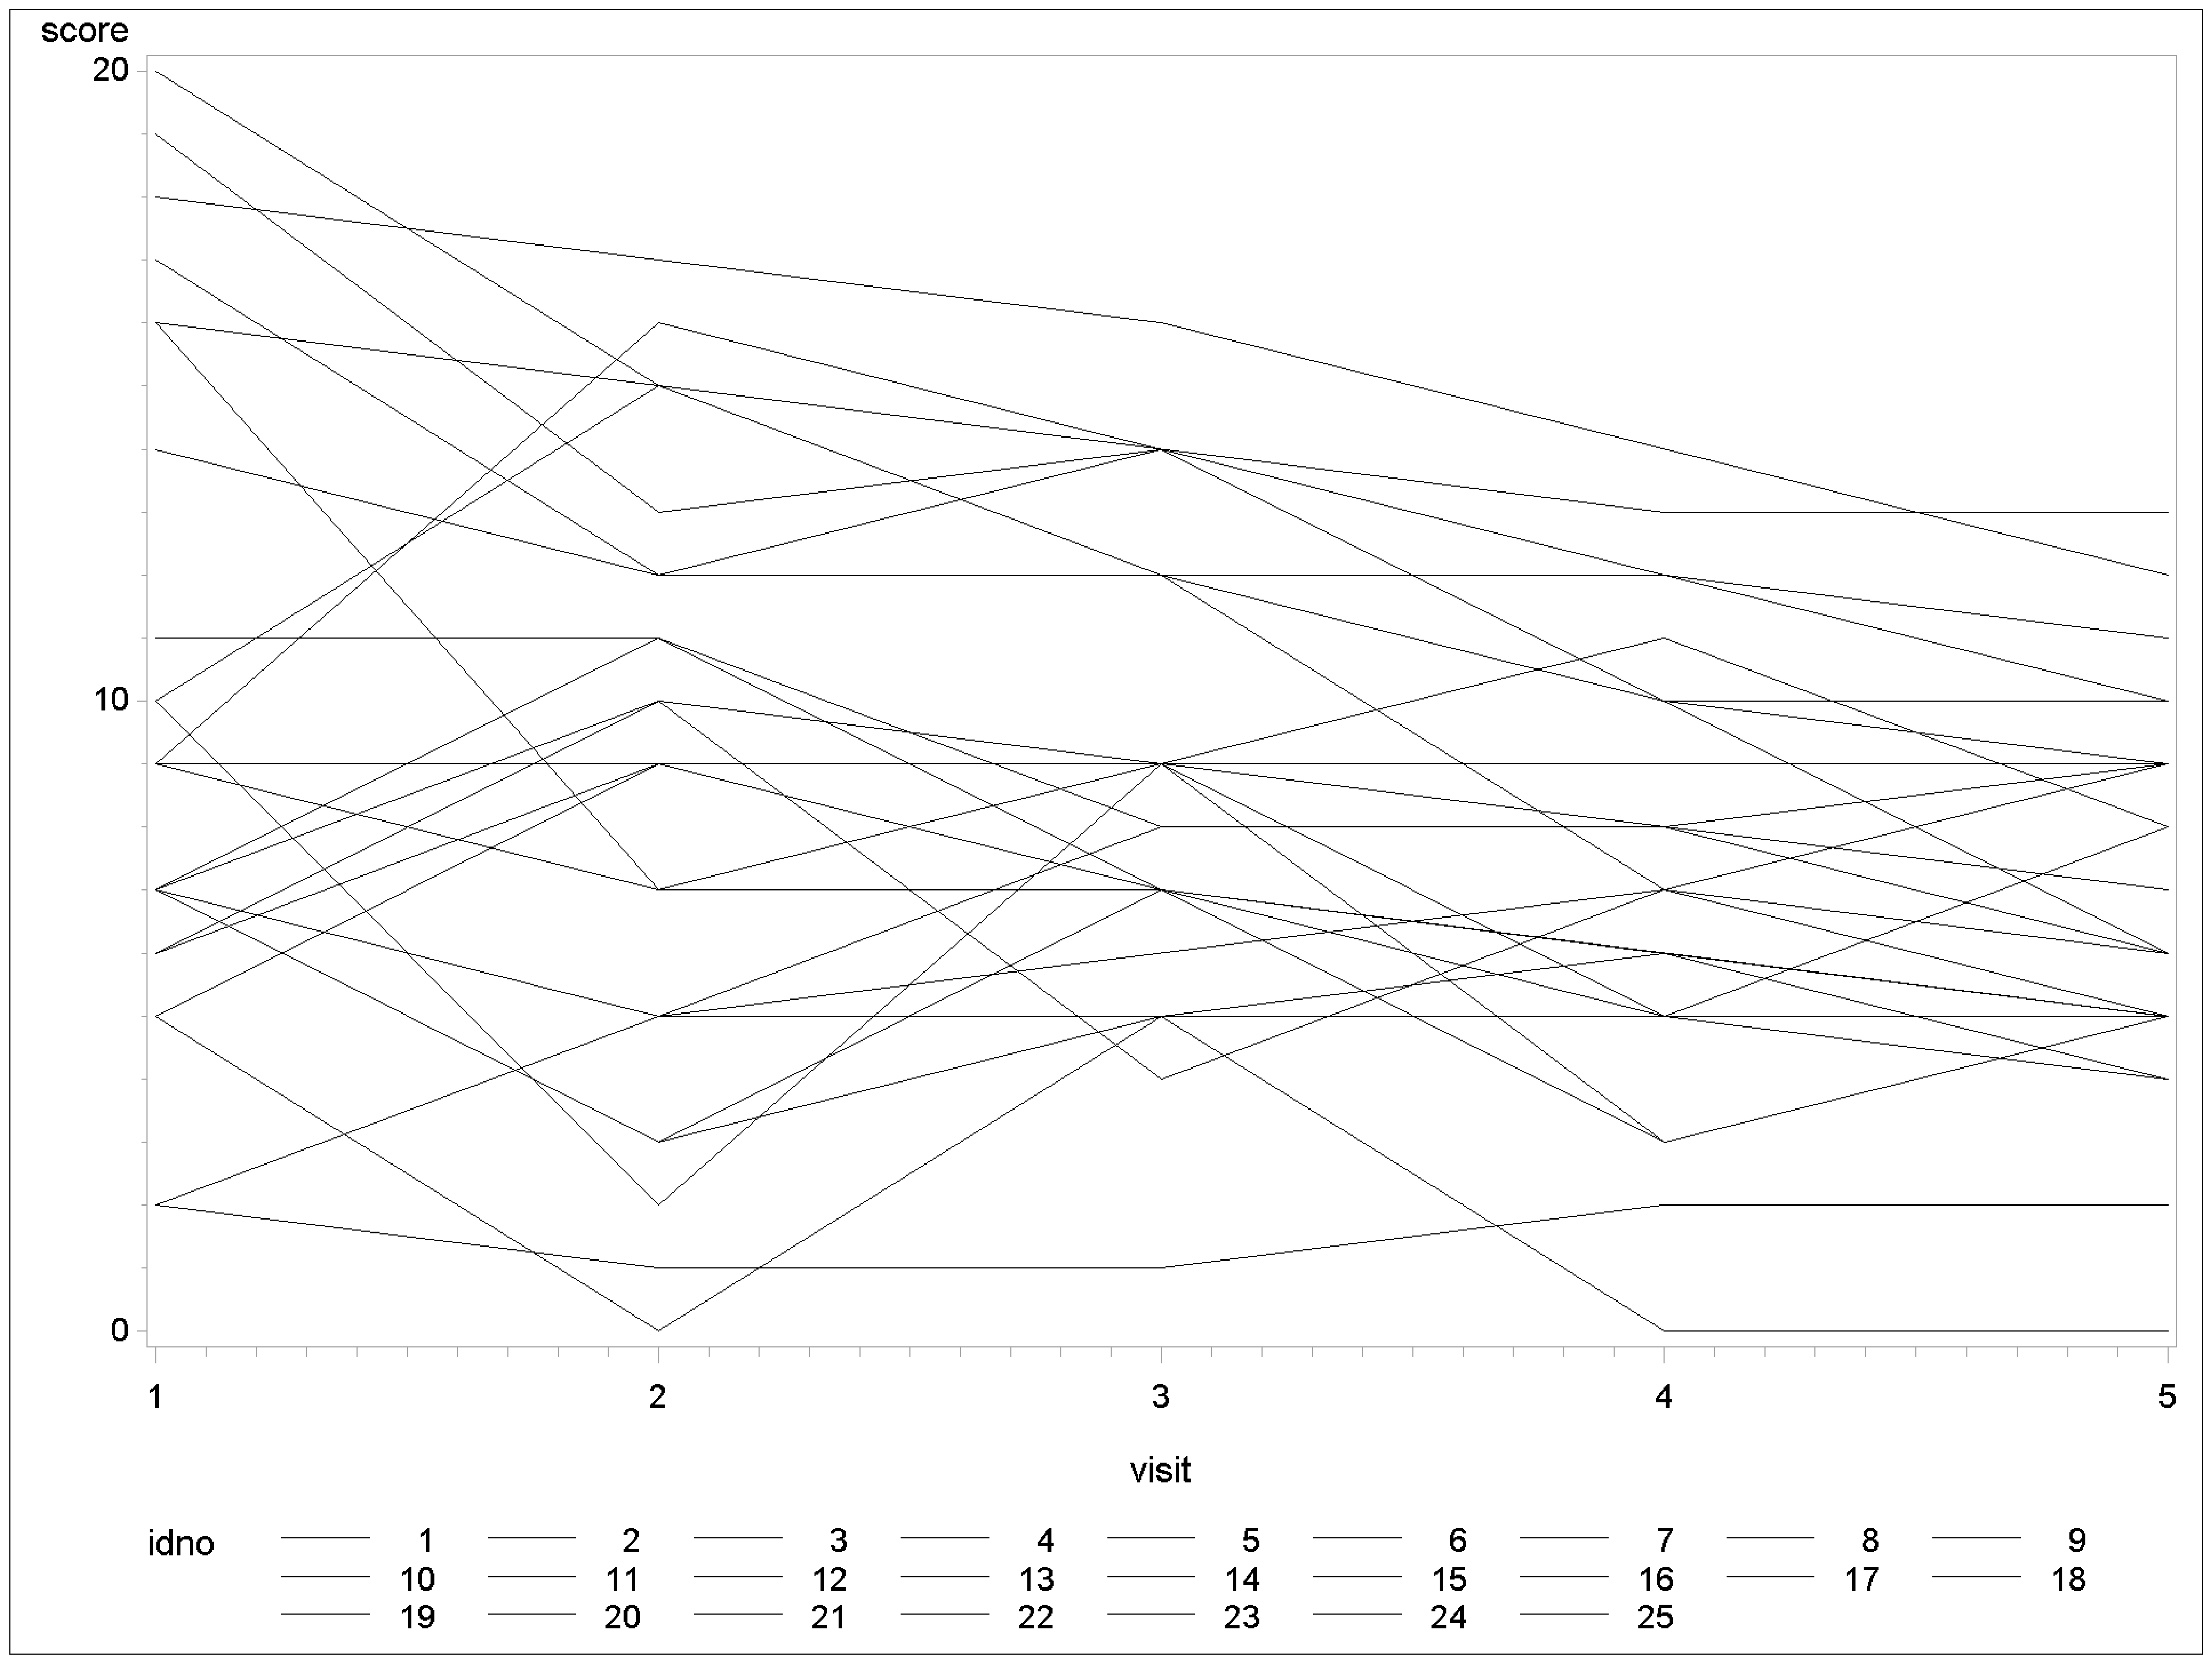
\includegraphics[width=2.4in]{h4re.eps}
		\end{minipage}
	}
	\subfigure[Subjects in Lecithin Group]{
		\begin{minipage}{0.4\textwidth}
			\centering
			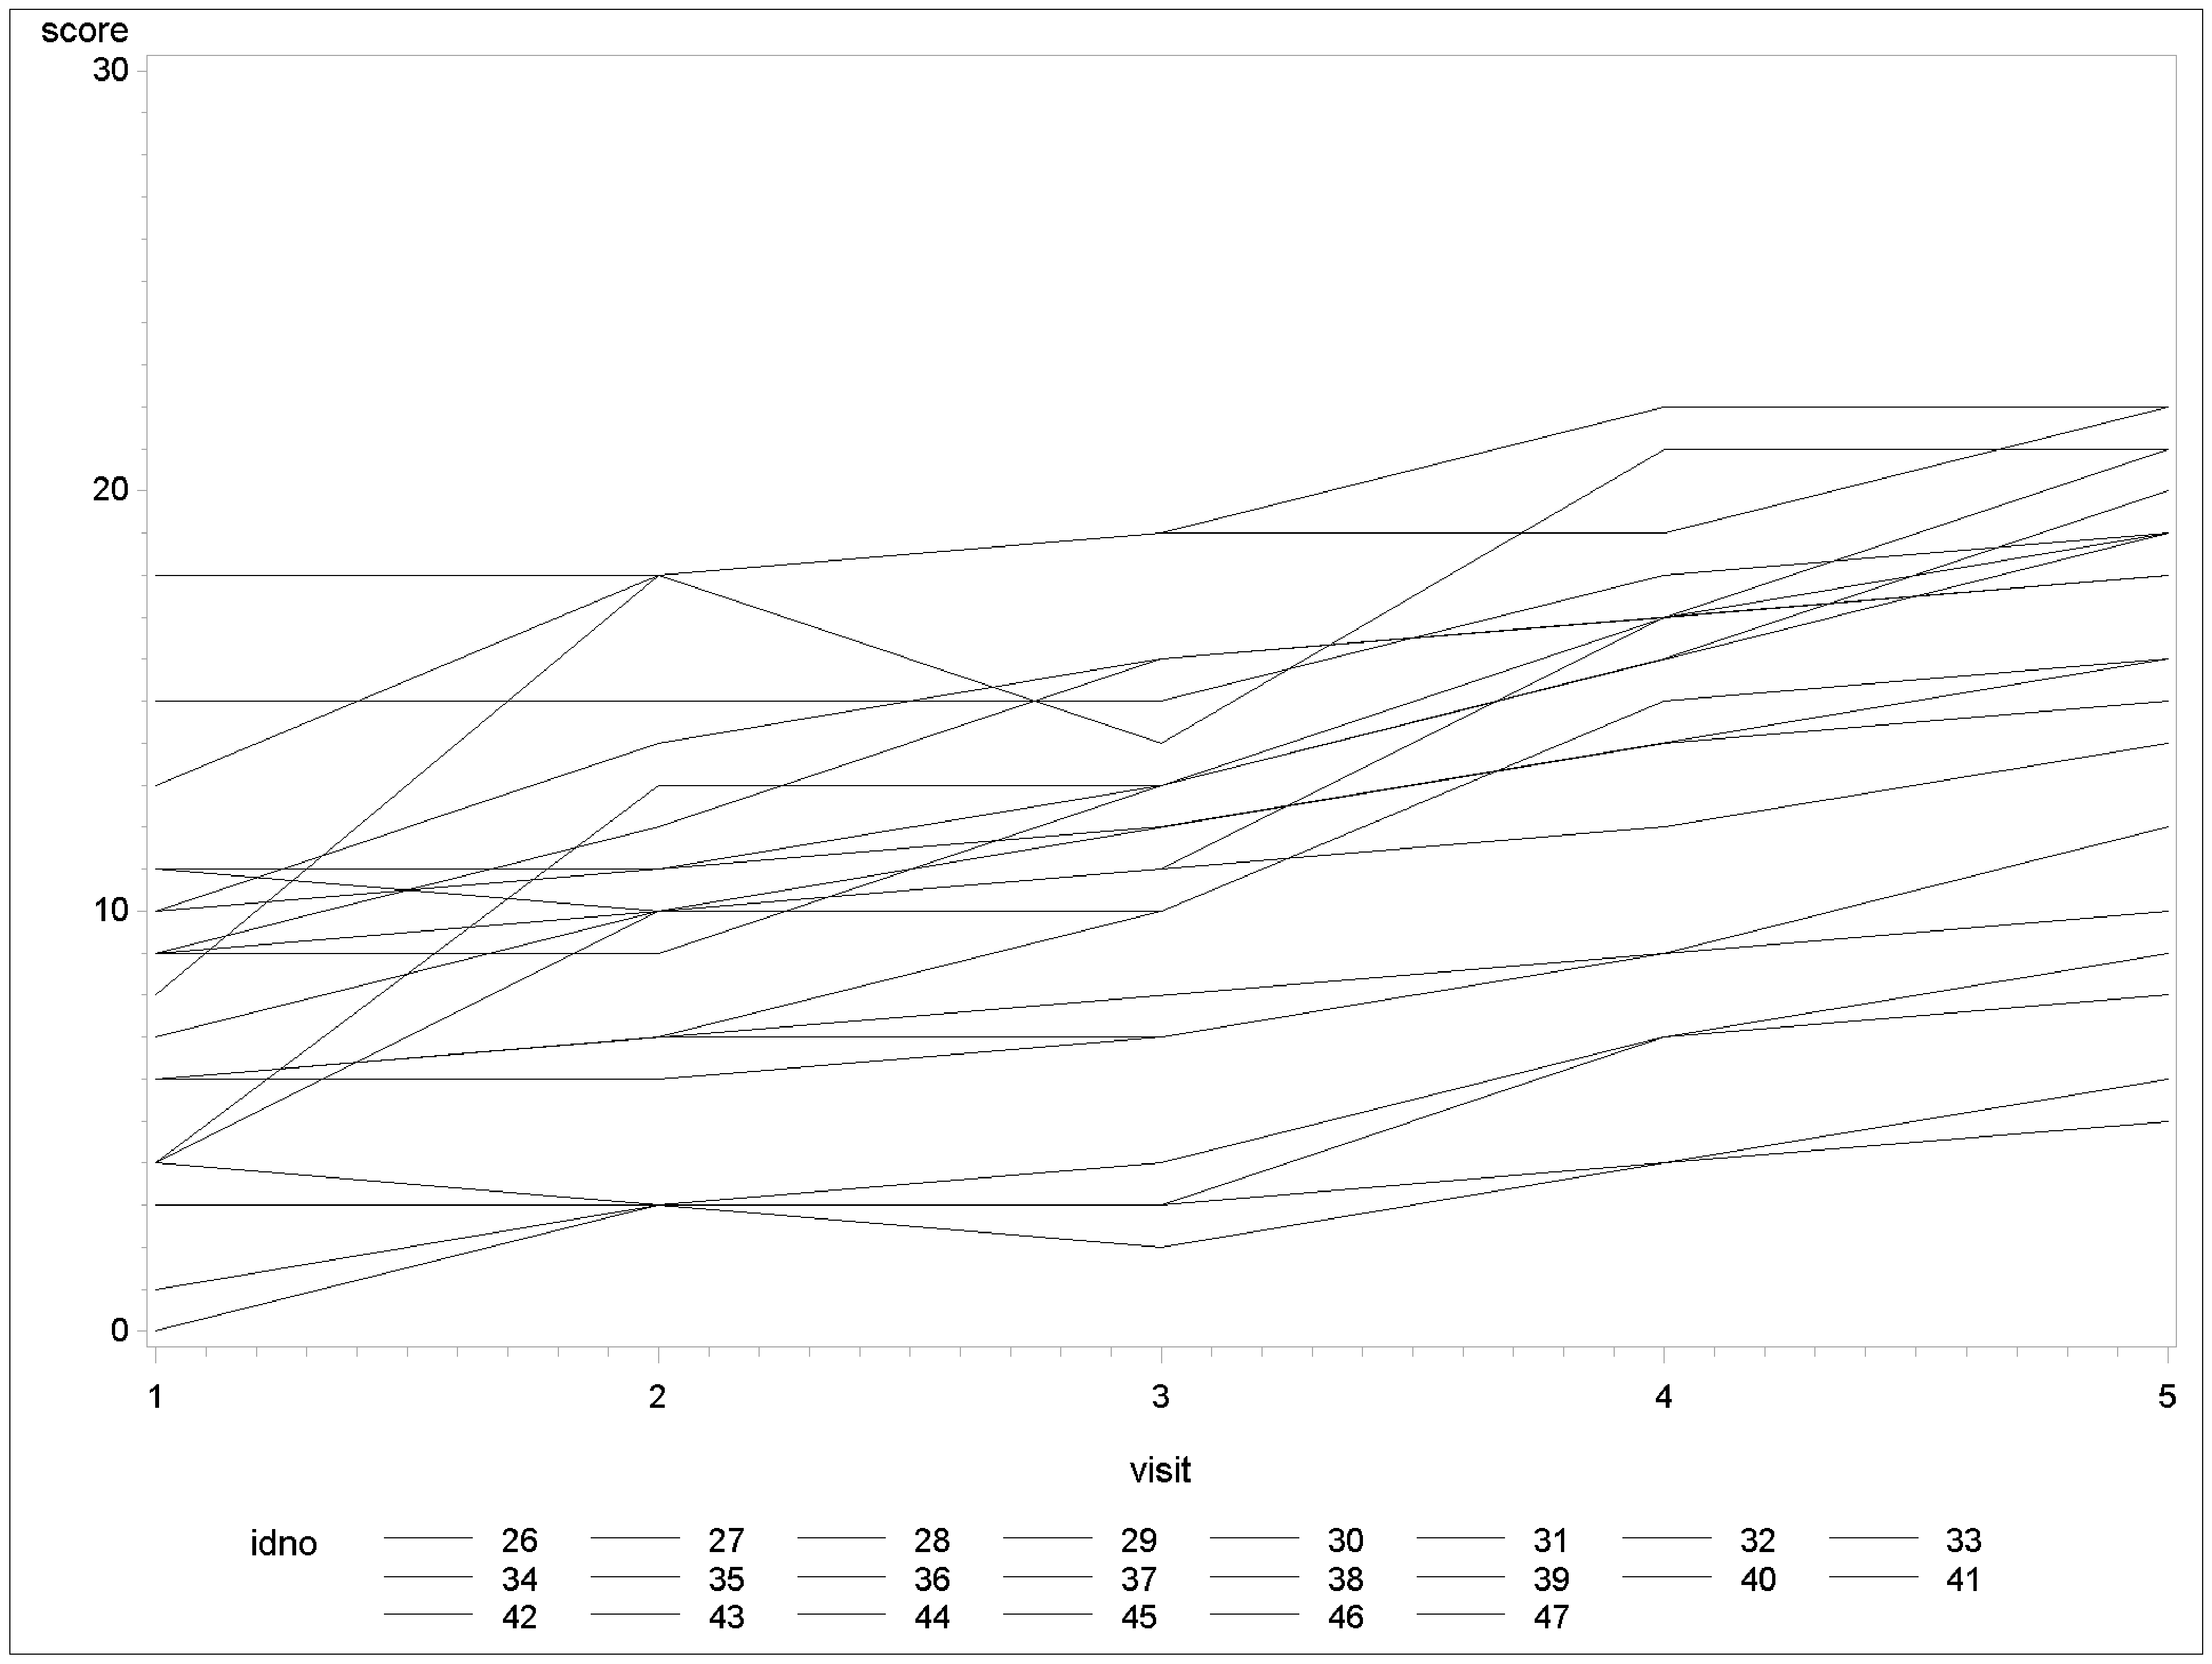
\includegraphics[width=2.4in]{h4re1.eps}
		\end{minipage}
	}
\end{figure}



(b). Firstly, we will define some notations. We denote $i$ as the index of group with $i=0,1$; $j$ as the index of visit with $j=1,2,3,4,5$ and $k$ as the index of subject with $k=1,2,\cdots,47$. $\bm{Y}_{k}=(y_{i1k},y_{i2k},y_{i3k},y_{i4k},y_{i5k})'$ denotes the repeated responses of a single subject. $X_1$ is a indictor variable of placebo group, where $X_{1}=1$ when the subject in placebo group. $X_2$ is a indictor variable of lecithin group, where $X_{2}=1$ when the subject in lecithin group. $t$ is treated as a continuous variable of visit. $X_1t$  and $X_2t$ denote the interaction of group and visit, which will show the different slopes of different groups. $\beta_0$ is the identical intercept, $\beta_1$ and $\beta_2$ are the coefficients of $X_1t$  and $X_2t$. $b_{0k}$ is the random component of the intercept, where $b_{0k}\sim \text{N}(0,\sigma_b^2)$. $\epsilon_{ijk}$ is error term, and $\epsilon_{ijk}\sim \text{N}(0,\sigma^2)$ Now we can construct the model based on the general structure,
$$
\bm{Y}_k=\bm{X_k\beta+Z_kb_k+\epsilon_k}
$$
where the $\bm{X\beta}$ are fixed effects, and $\bm{Zb}$ are random effects, and 
\begin{itemize}
\item $\bm{Y}_k=(y_{i1k},y_{i2k},y_{i3k},y_{i4k},y_{i5k})'$;
\item $\bm{X}_k=(\bm{1},\bm{X_1t},\bm{X_2t})=\lma
1&1&1&1&1\\
X_{1}&2X_{1}&3X_{1}&4X_{1}&5X_{1}\\
X_{2}&2X_{2}&3X_{2}&4X_{2}&5X_{2}\rma'$;
\item $\bm{\beta}=(\beta_0,\beta_1,\beta_2)'$;
\item $\bm{Z}_k=\bm{1}=(1,1,1,1,1)'$;
\item $\bm{b}_k=b_{0k}$.
\end{itemize}
We can also know that,
$$
var(\bm{b}_k)=\bm{D}=\sigma_b^2,\qquad var(\bm{\epsilon_k})=\bm{\Sigma}=\big\{_d\{_d \sigma^2\}_{j=1}^5\big\}_{k=1}^{25}
$$
where $\{_d \cdot\}$ denotes a diagonal matrix.

In this model, we assume that
\begin{itemize}
\item different groups have same intercept, that is, there exists significant;
\item intercept has random component;
\item $\bm{b}_k\sim\text{N}(\bm{0},\bm{D})$, $\bm{\epsilon}_k\sim\text{N}(\bm{0},\bm{\Sigma})$, that is, variance-covariance structure is VC(variance component), and residual structure is normal and independent;
\item the relationship between score and visit is linear.
\end{itemize}


(c). According to the model in part (2), we can get the marginal variance-covariance matrix of $\bm{Y}_k$ is 
$$
var(\bm{Y}_k)=\bm{ZDZ}'+\bm{\Sigma}=\sigma_b^2\bm{ZZ}'+\bm{\Sigma}=\lma
\sigma^2_b+\sigma^2&\sigma^2_b&\cdots&\sigma^2_b\\
\sigma^2_b&\sigma^2_b+\sigma^2&\sigma^2_b&\cdots\\
\vdots&\vdots&\ddots&\vdots\\
\sigma^2_b&\cdots&\cdots&\sigma^2_b+\sigma^2\rma_{5\times 5}
$$


(d). To fit the model, the SAS code is as blow,
\begin{Sascode}[store=class]
proc mixed data=alzheim method=ml noitprint;
class idno group;
model score=group*visit/ s outp=rdint;
random int/subject=idno;
run;
\end{Sascode}

\begin{enumerate}[i.]
\item The estimates for variance components are
$$
\sigma_{b}^2=20.0242,\quad \sigma^2=4.0691
$$

\item What we want to test is
$$
H_0:\beta_1=\beta_2\quad\text{v.s.}\quad H_a: \beta_1\not=\beta_2
$$
From the Type 3 test of fixed model, we have a significant P-value which is less than 0.0001. So we we reject null hypothesis, and get $\beta_1\not=\beta_2$ which means that treatment effect is significant. And from the estimates, we have $\beta_1=-0.6133<1.7514=\beta_2$, which means the scores in the lecithin group are increasing over time, while scores in placebo are decreasing. thus, treatment helps.

\item From the plots (Firgure \ref{plot2}), firstly it shows the differences of slopes of groups, or in another word, the difference of treatment effects. Secondly, it shows that the status of patients are different at the initial of the experiment, which causes the different intercepts of the regression lines. However, from the graphs, the reactions of patients under the same treatment seem same, because different lines in same group have same slope. This is not so realistic, since we know that the difference of patient's physical or mental status may also cause the effect of treatment to be different. So the different lines should have different slopes.
\end{enumerate}
\begin{figure}[htbp]
	\caption{Plots by Group with Random Intercept}
	\label{plot2}
	\centering
	\subfigure[Subjects in Placebo Group]{
		\begin{minipage}{0.4\textwidth}
			\centering
			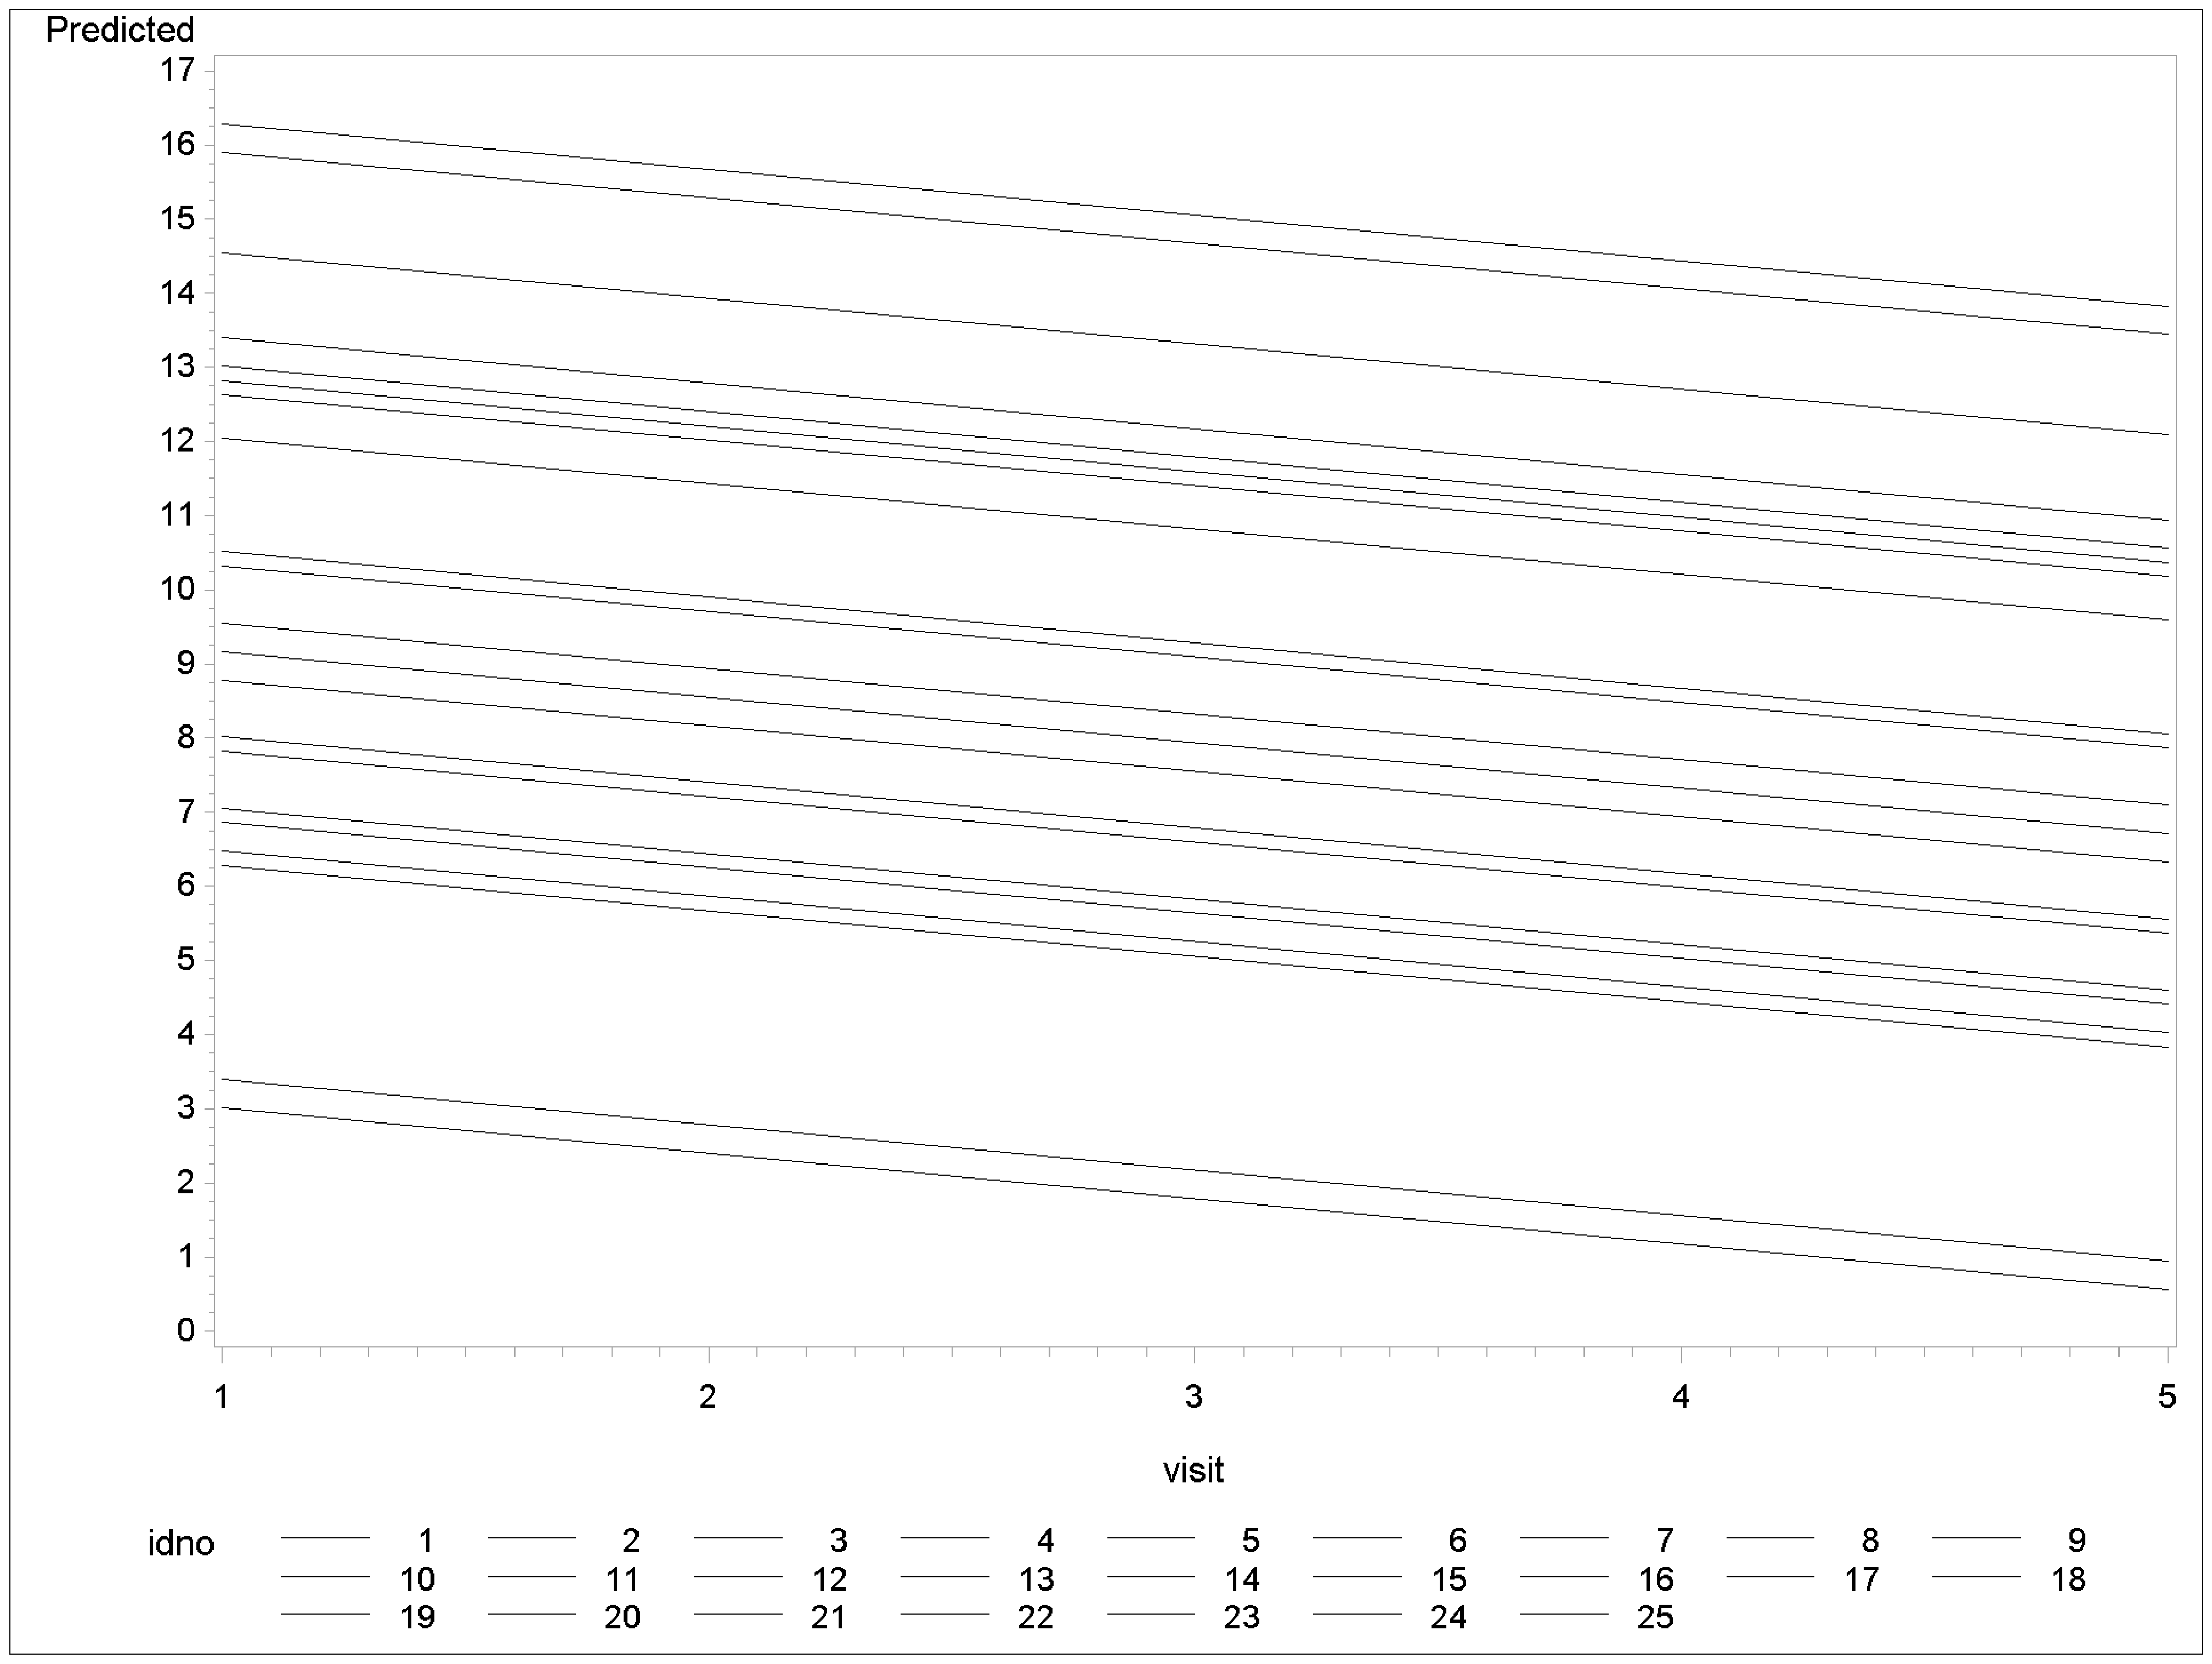
\includegraphics[width=2.4in]{h4re2.eps}
		\end{minipage}
	}
	\subfigure[Subjects in Lecithin Group]{
		\begin{minipage}{0.4\textwidth}
			\centering
			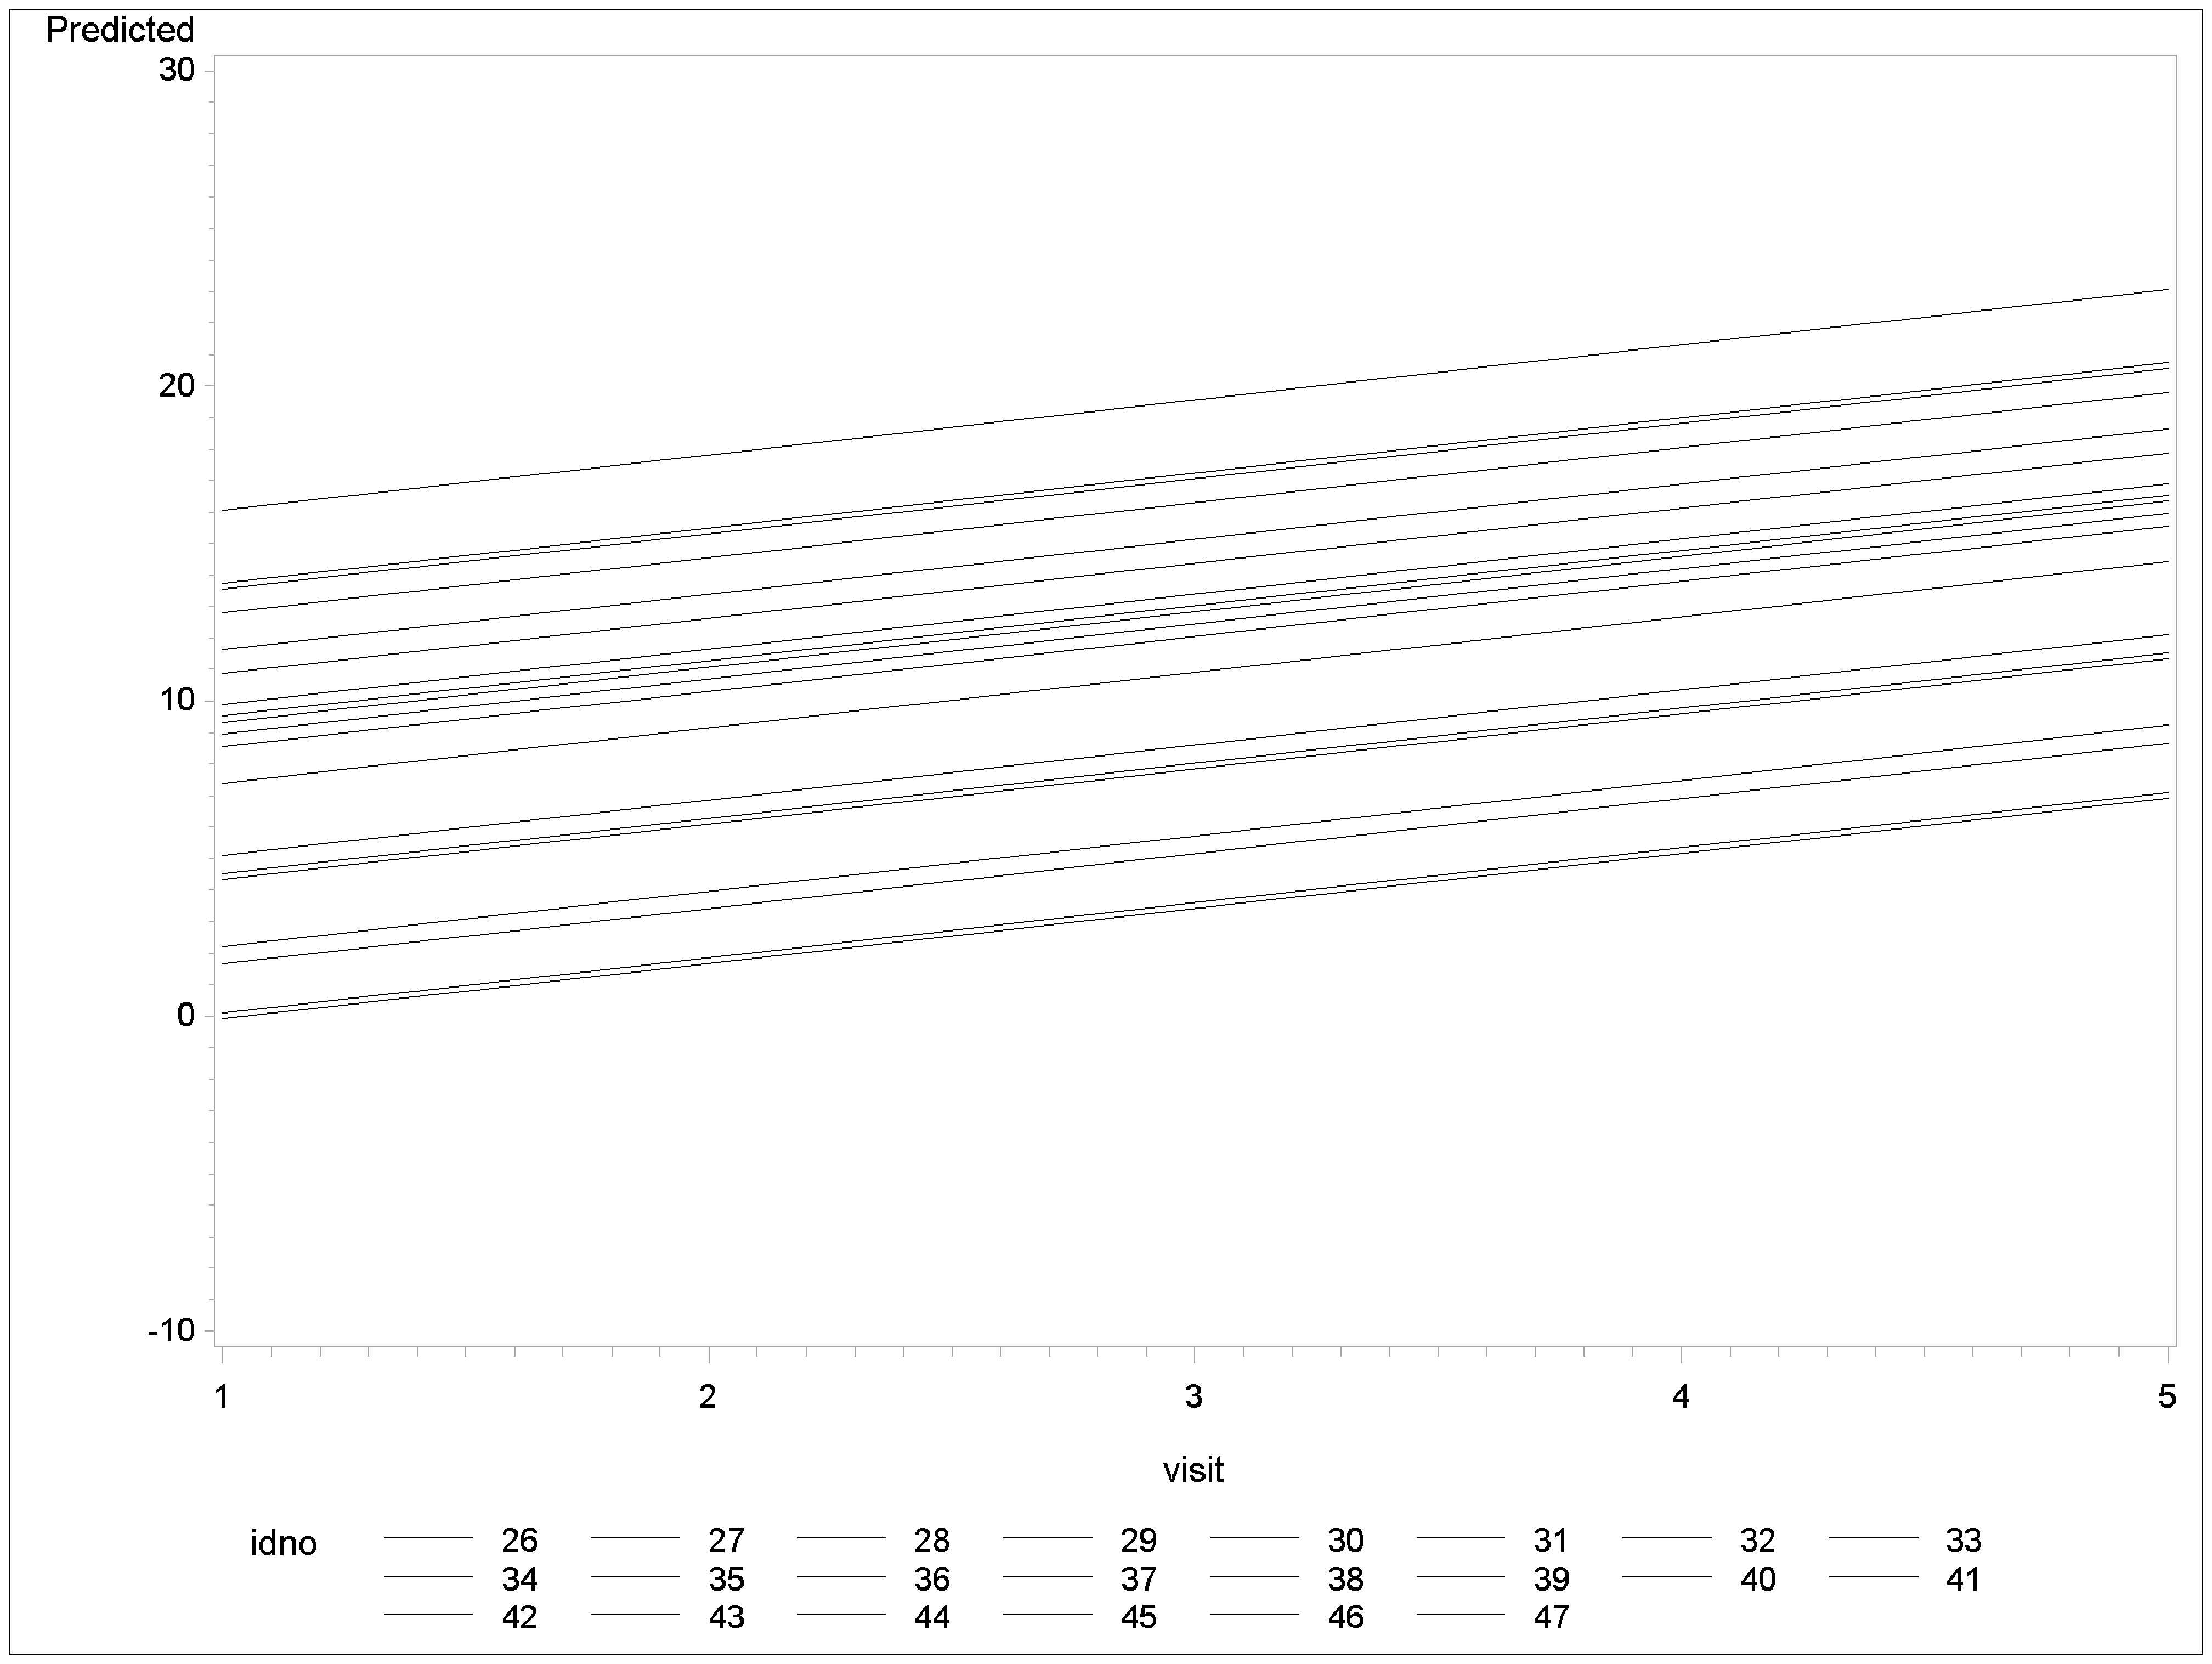
\includegraphics[width=2.4in]{h4re3.eps}
		\end{minipage}
	}
\end{figure}


(e). We can rewrite the model in part (b),
$$
\bm{Y}_k=\bm{X_k\beta+Z_kb_k+\epsilon_k}
$$
The only differences here from part (b) are
$$
\bm{Z}_k=\lma 1&1&1&1&1\\1&2&3&4&5\rma';\quad
\bm{b}_k=(b_{0k},b_{1k})'.
$$
and
$$
var(\bm{b}_k)=\bm{D}=\lma d_{11} &d_{12}\\d_{21}&d_{22}\rma
$$
The assumptions of this model almost same, but we also need to assume that the coefficients also have random components.


(f). The SAS code is as blow,
\begin{Sascode}[store=class]
proc mixed data=alzheim method=ml noitprint covtest;
class idno group;
model score=group*visit/ s outp=rdcoe;
random int visit/subject=idno type=un;
run;
\end{Sascode}

\begin{enumerate}[i.]
\item The estimates for variance components are
\ba
var(\bm{b})&=\lma 26.2524&-1.8274\\-1.8274&0.4208\rma\\
\sigma^2&=3.1035
\ea
The P-value of $d_{11}$ is less the 0.0001, the P-value of $d_{12}=d{21}=0.296$, the P-value of $d_{22}$ is 0.0049 and the P-value of $\sigma$ is less than 0.0001. Thus, all variance components are significant. The correlation between intercepts and slopes is
$$
corr(\beta_{0k},\beta_{1k})=\frac{cov(\beta_{0k},\beta_{1k})}{\sqrt{var(\beta_{0k})}\sqrt{var(\beta_{1k})}}=\frac{-1.8274}{\sqrt{26.2524}\sqrt{0.4208}}=-0.5498
$$

\item What we want to test is
$$
H_0:\beta_1=\beta_2\quad\text{v.s.}\quad H_a: \beta_1\not=\beta_2
$$
From the Type 3 test of fixed model, we still have a significant P-value which is less than 0.0001. So we we reject null hypothesis, and get $\beta_1\not=\beta_2$ which means that treatment effect is significant. And from the estimates, we have $\beta_1=-0.5173<1.6424=\beta_2$, thus, the treatment helps. This is a same result from part (d), just different estimations of parameters when adjusted by randomness of subject.

\item To compare the fitness of models, we can perform a likelihood ratio test,
$$
H_0:\text{ Reduced Model in part (b)}\quad\text{v.s.}\quad H_a:\text{ Full Model in part (e)}
$$
In the reduced model, we have $d_{12}=0$ and $d_{22}=0$.
The statistic is 
$$
\Lambda=-2(\ell(Reduced~Model)-\ell(Full~Model))=1149.1-1134.8=14.3\sim\chi^2(2)
$$
The critical value of $\chi^2_{0.95}(2)$ is 5.99, which is less than 14.3. And the P-value is 0.0008. So we reject the null hypothesis. It is reasonable to believe that the model with random coefficient and unstructured variance-covariance structure is better fit than the random intercept model.
\item From the plots (Firgure \ref{plot3}), the different lines have different slopes compared with the parallel lines in the plots of random intercept model. It is more like the data plot, so we can think that it is a more realistic model.
\end{enumerate}
\begin{figure}[htbp]
	\caption{Plots by Group with Random Intercept and Coefficients}
	\label{plot3}
	\centering
	\subfigure[Subjects in Placebo Group]{
		\begin{minipage}{0.4\textwidth}
			\centering
			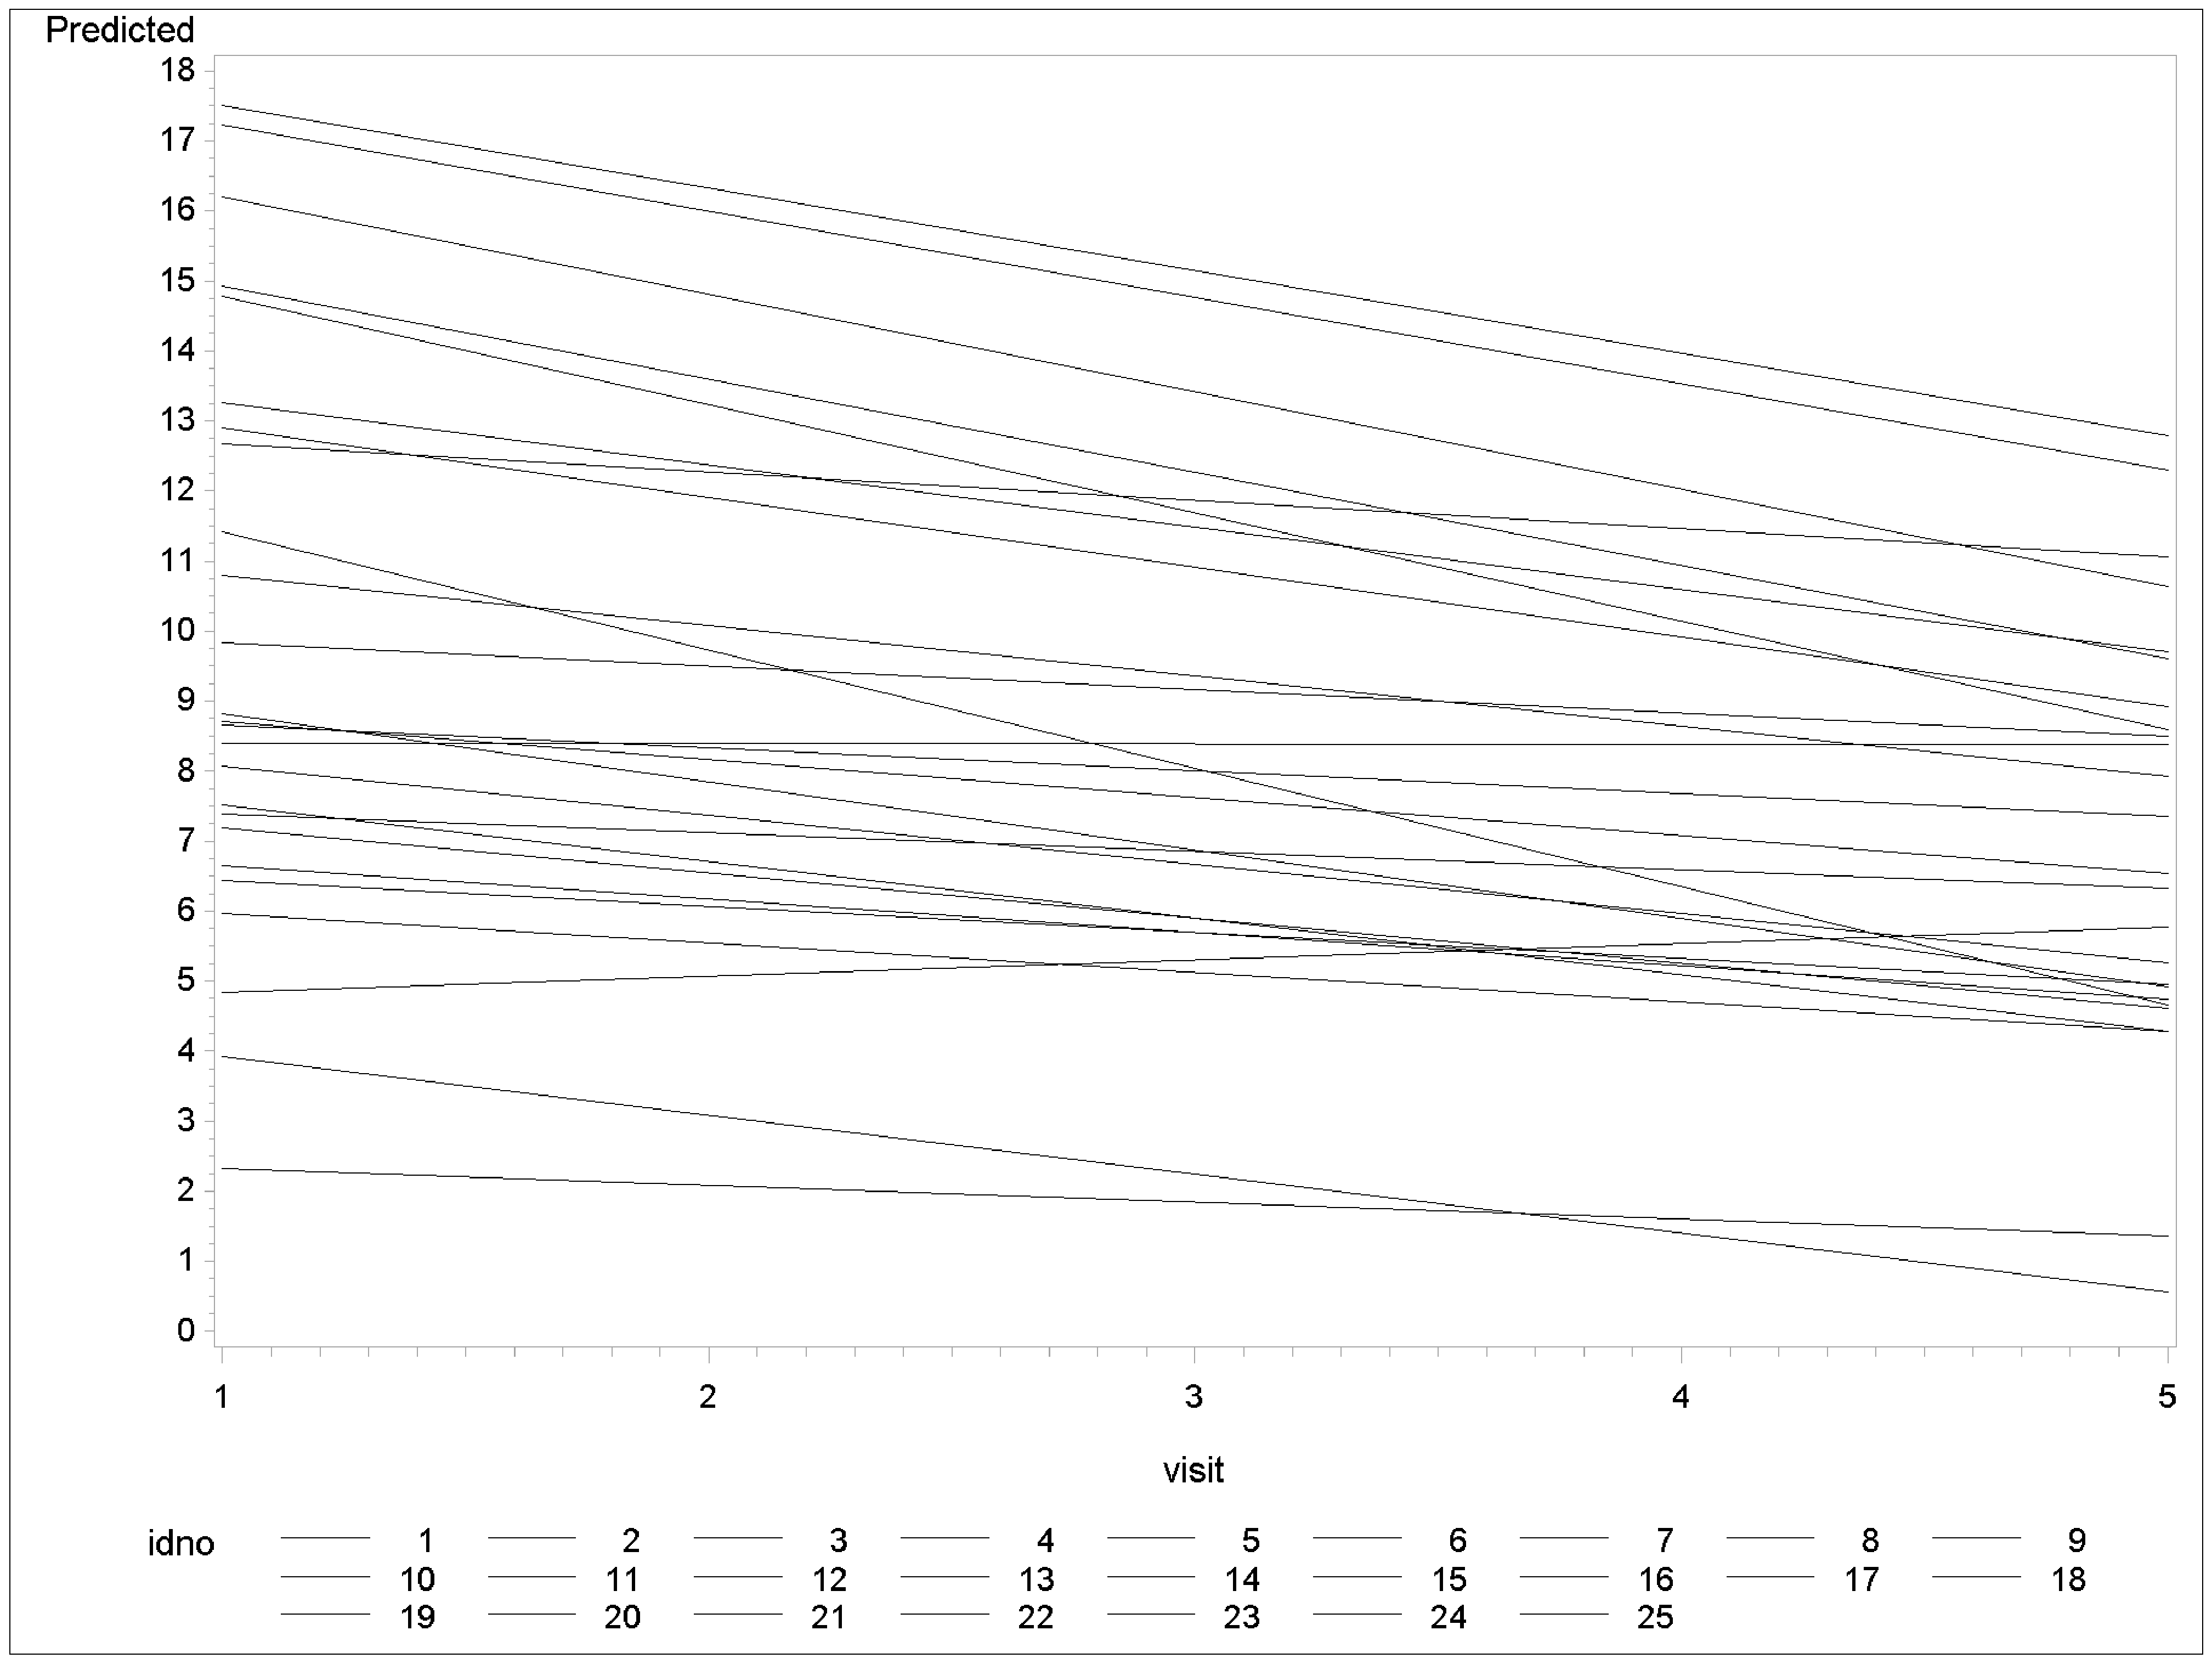
\includegraphics[width=2.4in]{h4re4.eps}
		\end{minipage}
	}
	\subfigure[Subjects in Lecithin Group]{
		\begin{minipage}{0.4\textwidth}
			\centering
			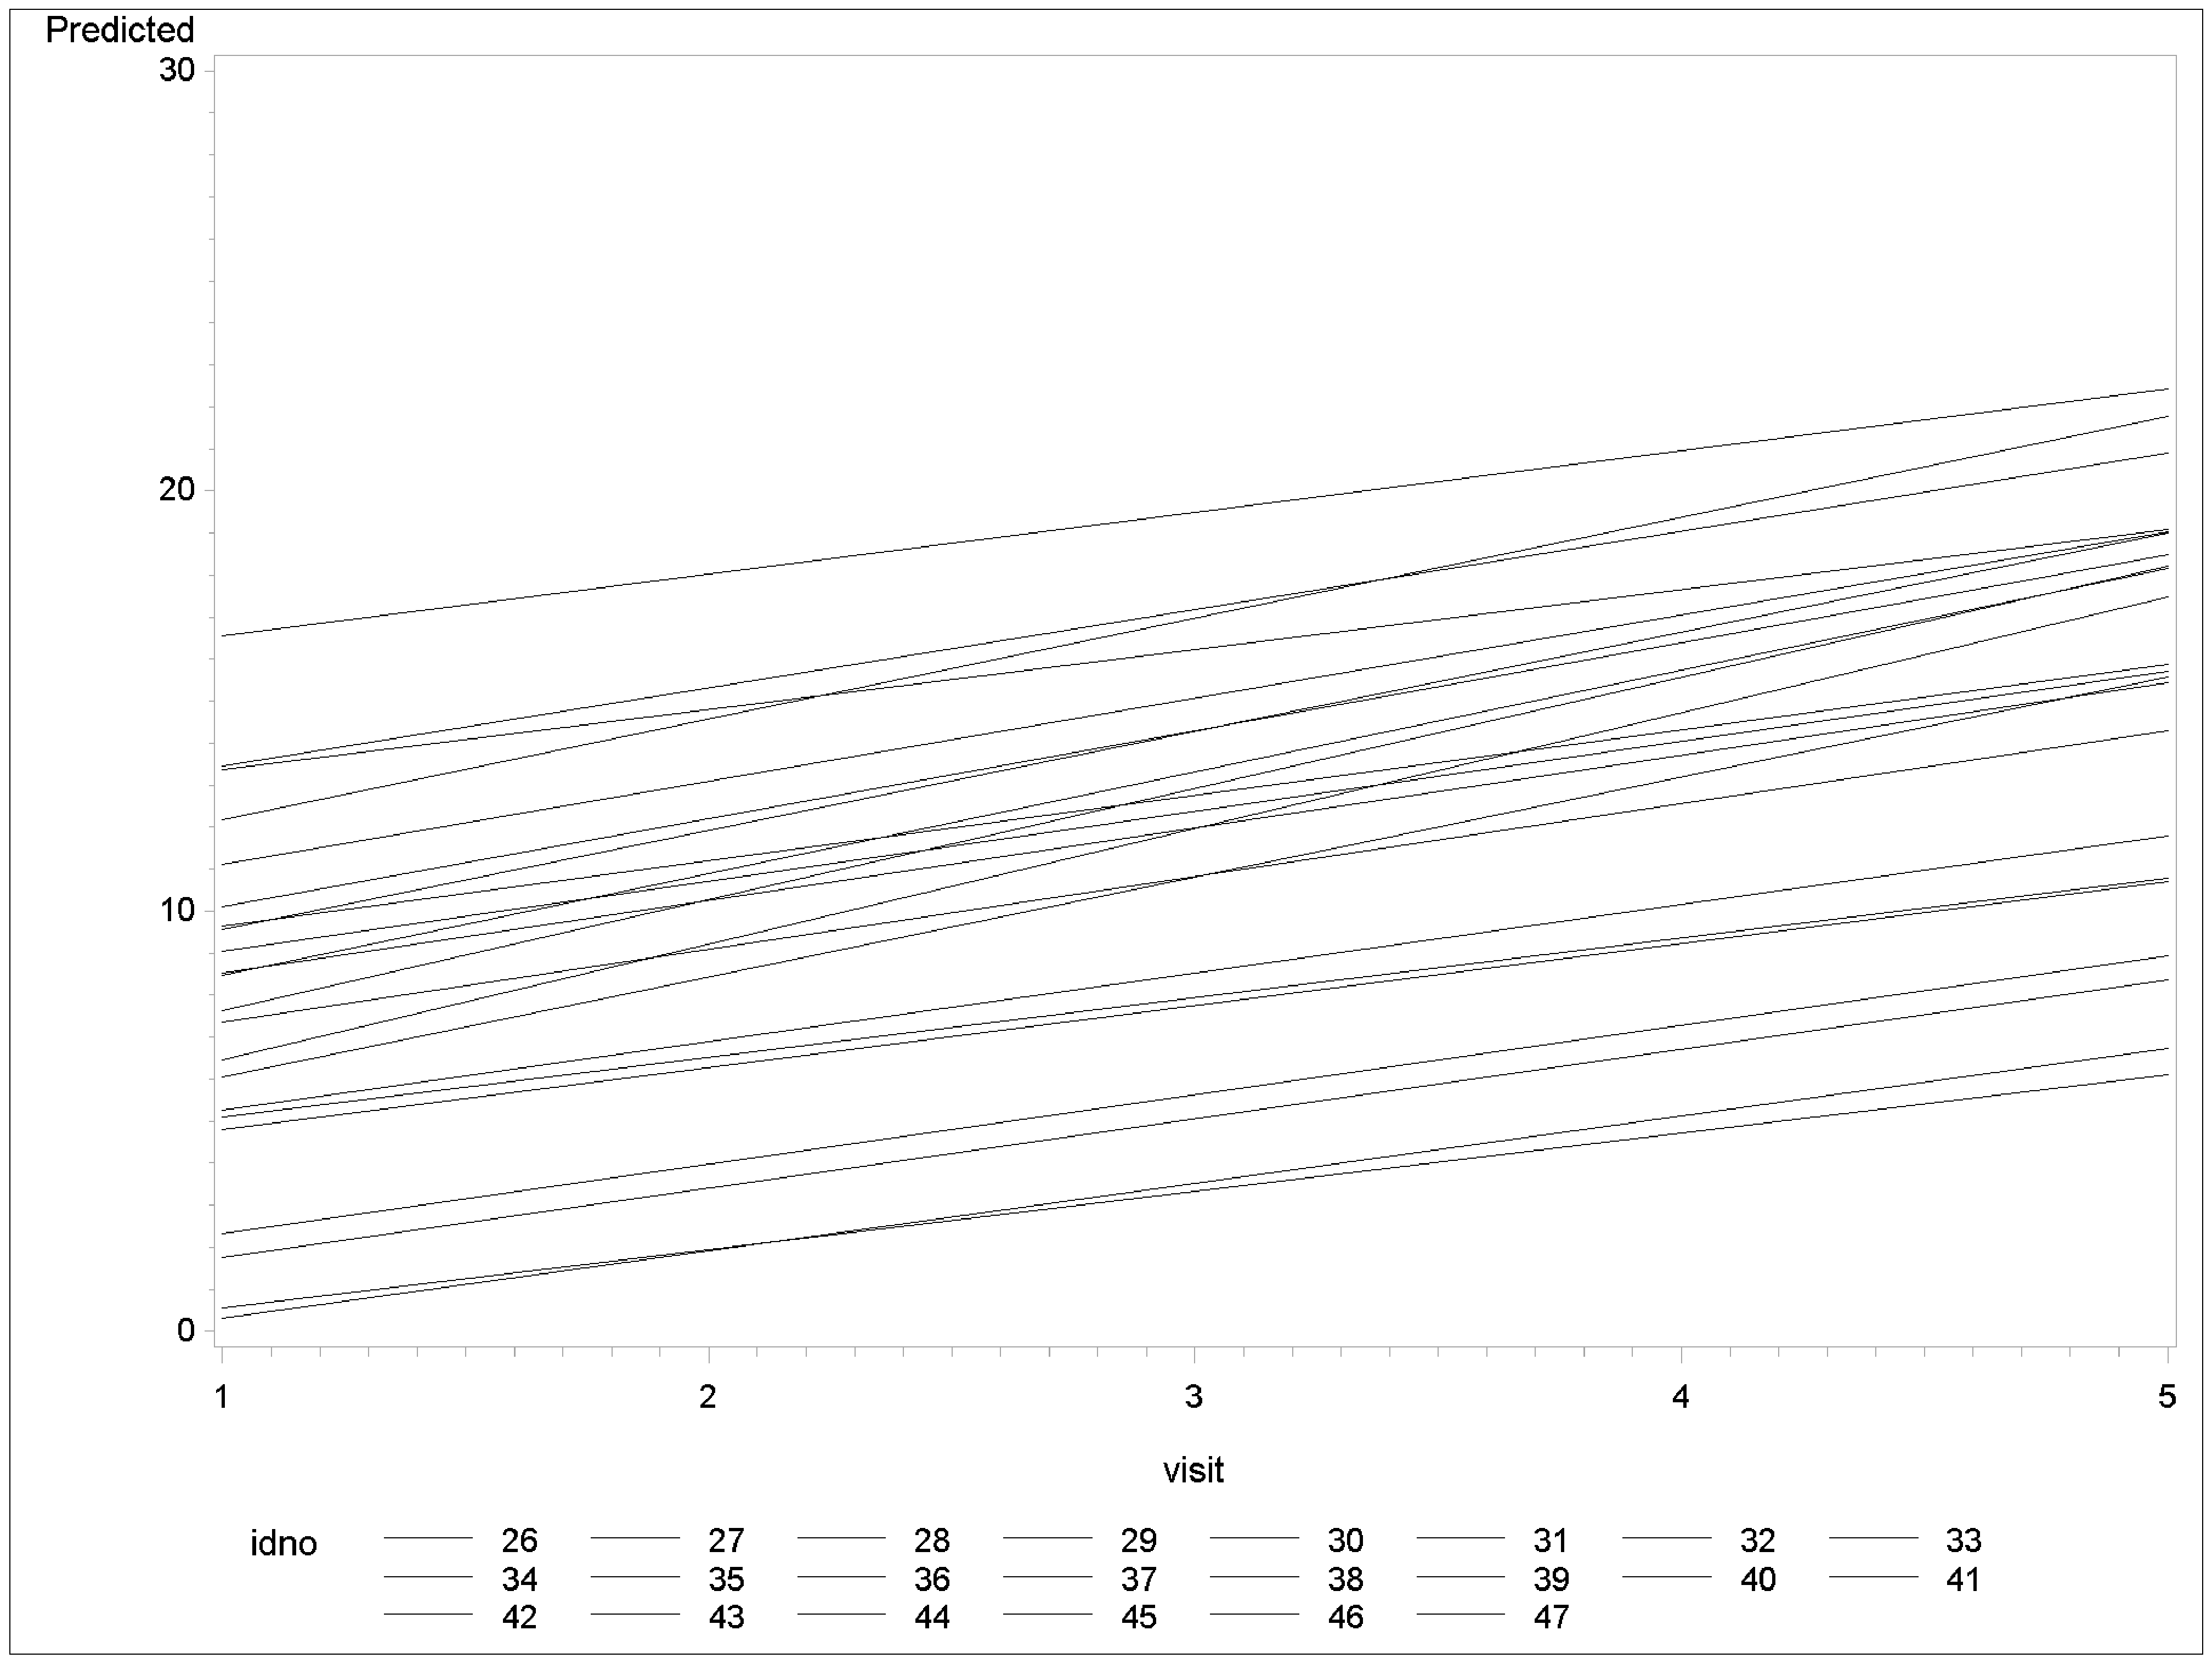
\includegraphics[width=2.4in]{h4re5.eps}
		\end{minipage}
	}
\end{figure}


(g). First, we should change the form of the model in part (e), 
$$
\bm{Y}_k=\bm{X_k\beta+e_k}
$$
Here, we put the random effect $\bm{Z_kb_k}$ and residual $\epsilon_k$ together to create the new residual side matrix. This time we want to control the residual matrix directly, other than the variance-covariance matrix of random effect. So here, we will define
$$
\bm{e}_k\sim\text{N}(\bm{0},\bm{\Sigma}_k^2),\ \ \text{where the structure of }\bm{\Sigma}_k^2\text{ is unknown}
$$

To refit the model assuming the residual side matrix structure is the first order autoregression or unstructured covariance. we use the code below using SAS,
\begin{Sascode}
proc mixed data=alzheim noitprint contest;
class group visit;
model score=group|visit/ s outp=repmar;
repeated visit / subject=idno type=ar(1);
run;

proc mixed data=alzheim noitprint covtest;
class idno group visit;
model score=group|visit/ s outp=repun;
repeated visit / subject=idno type=un;
run;
\end{Sascode}


For repeated measures model here, it is more like a nested experimental design, since it does not focus on the form of the relation between scores and visit, but just to compare the difference between scores under different combinations of group and visit. So SAS will give us 10 fixed parameter estimates rather than 3 (2 slopes and 1 intercept) as before. For the first order autoregression structure, we will get the estimate of correlation coefficient between two sequential visits
$$
\rho=0.8422,\quad\text{with the P-value}<0.0001
$$
The significant correlation coefficient implies that the score is related with the previous score, so the independent assumption may not be appropriate.


So the residual variance-covariance matrix is
$$
\bm{\Sigma}_k=\lma
20.8085 &17.5250 &14.7596 &12.4306 &10.4691 \\
17.5250 &20.9095 &17.5250 &14.7596 &12.4306 \\
14.7596 &17.5250 &20.9095 &17.5250 &14.7596 \\
12.4306 &14.7596 &17.5250 &20.9095 &17.5250 \\
10.4691 &12.4306 &14.7596 &17.5250 &20.9095 
\rma
$$
while the marginal variance-covariance matrix of iid error model is
\ba
\bm{V}&=\bm{ZDZ}'+\bm{\Sigma}\\
&=\lma
26.1219 &21.6118 & 20.2052 &18.7986 &17.3920\\
21.6118 &23.7295 & 19.6402 &18.6544& 17.6686\\
20.2052 &19.6402& 22.1787 &18.5102& 17.9452\\
8.7986 &18.6544 &18.5102 &21.4695 &18.2218\\
17.3920 &17.6686& 17.9452 &18.2218& 21.6019\\
\rma
\ea
There is no surprising that they are different. As mentioned before, the repeated measure model is more like ANOVA, so here we should firstly test the interaction effect,
$$
H_0:~\text{The interaction is insignificant}\quad\text{v.s.}\quad H_a:~\text{The interaction is significant}
$$
then the interaction have s significant P-value less than 0.001. With significant interaction effect, we cannot test the main effect of group. But we can contrast them
$$
H_0:\mu_\text{group 1}-\mu_\text{group 2}=0\quad\text{v.s.}\quad H_a:\mu_\text{group 1}-\mu_\text{group 2}\not=0
$$
The absolute difference is 3.0556 with P-value=0.0125, thus, we can still say that the treatment helps. Moreover the -2 times REML, AIC and BIC of AR(1) model is better than the model in part (e). Thus, we can believe that AR(1) model here is a better model than iid models. (Here we cannot perform a likelihood ratio test to support our conclusion, because these two models are not nested models)

Finally, we refit the repeated measure model by assuming unstructured covariance as the code above. We can see that the AIC of AR(1) model is 1148.8, while AIC of UN model is 1097.1. Thus we may choose unstructured model as a more appropriate. This also gives us a hint that the assumption of first order autoregression correlation structure may be not the real correlation of this longitude data, the correlation structure may be more complicated.







%\Listing[store=class,
%  caption={Regression Analysis}]{resultl}

%\Graphic[store=class, scale=0.9,
%  caption={Graphs for Regression Analysis}]{resultg}

\end{document}
